\begin{figure}[ht]
  \centering
  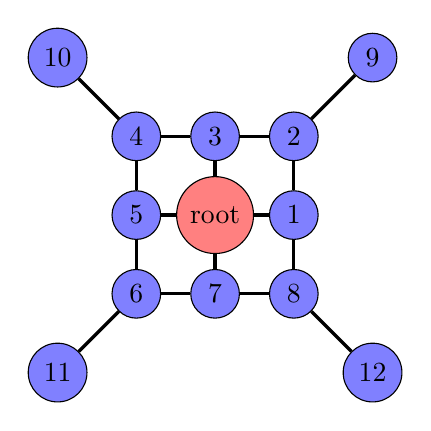
\begin{tikzpicture}
  % définition des styles
  \tikzstyle{root}=[circle, draw, fill=red!50,text=black]
  \tikzstyle{node}=[circle, draw, fill=blue!50,text=black]

  \tikzstyle{estun}=[-,>=latex,very thick]
  % les nœuds
  \node[root] (root) at (0, 0) {root};

  \node[node] (1) at (1,0) {1};
  \node[node] (2) at (1,1) {2};
  \node[node] (3) at (0,1) {3};
  \node[node] (4) at (-1, 1) {4};
  \node[node] (5) at (-1, 0) {5};
  \node[node] (6) at (-1, -1) {6};
  \node[node] (7) at (0, -1) {7};
  \node[node] (8) at (1, -1) {8};

  \node[node] (9) at (2, 2) {9};
  \node[node] (10) at (-2, 2) {10};
  \node[node] (11) at (-2, -2) {11};
  \node[node] (12) at (2, -2) {12};

  \draw[estun] (root)--(1);
  \draw[estun] (root)--(3);
  \draw[estun] (root)--(5);
  \draw[estun] (root)--(7);

  \draw[estun] (1)--(2);
  \draw[estun] (2)--(3);
  \draw[estun] (3)--(4);
  \draw[estun] (4)--(5);
  \draw[estun] (5)--(6);
  \draw[estun] (6)--(7);
  \draw[estun] (7)--(8);
  \draw[estun] (8)--(1);

  \draw[estun] (2)--(9);
  \draw[estun] (4)--(10);
  \draw[estun] (6)--(11);
  \draw[estun] (8)--(12);

  \end{tikzpicture}

  \caption{Topologie radio considérée pour la validation expérimentale du \ac{RPCA}.}

  \label{cache:fig:topology}
\end{figure}
